%\usepackage{amsmath}
%\usepackage{hyperref}
%\usepackage{amsthm}
%\usepackage{graphicx}
\documentclass[journal, a4paper]{IEEEtran}
\usepackage[italian]{babel}
\usepackage{booktabs}
\usepackage{siunitx}%Questo serve a caricare il pacchetto delle unità di misura del sistema internazionale%
\usepackage[utf8]{inputenc}
\usepackage{graphicx} 
\usepackage{url}
\usepackage{amsmath}
\usepackage{amssymb}


\usepackage{keyval}
\usepackage{xcolor}
\usepackage{caption}
\usepackage{tikz}
\usepackage{circuitikz}
\usepackage{authblk}
%\usepackage{hyperref}

\begin{document}


% Define document title and author
	\title{Tecnologie Digitali - Logbook Week 8}
	\author[1]{Salvatore Bottaro}
		\author[2]{Lorenzo M. Perrone}
		\affil[1]{\texttt{salvo.bottaro@hotmail.it}}
		\affil[2]{\texttt{lorenzo.perrone.lmp@gmail.com}}
	\markboth{Tecnologie Digitali - Di Lieto}{}
	\maketitle
	
\begin{abstract}
	Logbook di laboratorio di Tecnologie Digitali, a.a. 2015/2016. Week 8.
\end{abstract}

Le celle fotovoltaiche al silicio consentono di convertire in corrente elettrica la radiazione luminosa incidente. La responsività spettrale dipende dalla struttura cristallina del silicio.

\subsection{Hm. 1}

Come si vede in figura \ref{fig:silres1} e \ref{fig:silres2}, il silicio amorfo è in grado di convertire in corrente elettrica fotoni con lunghezza d'onda fra i 350 e 800 nm, con un picco di responsività sul giallo-verde, mentre il silicio cristallino copre un più ampio spettro da 350 nm a 1200 nm, con picco per lunghezze d'onda intorno ai 900 nm.

\begin{figure}[htp]
\centering
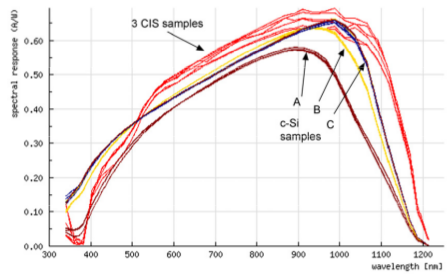
\includegraphics[scale=.5]{c-Si_SR}
\caption{Responsività spettrale di celle fotovoltaiche con silicio amorfo e monocristallino.}
\label{fig:silres1}
\end{figure}

\begin{figure}[htp]
\centering
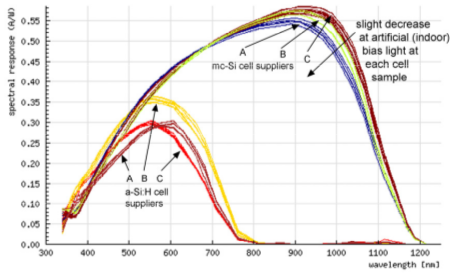
\includegraphics[scale=.5]{mc-Si_SR}
\caption{Responsività spettrale di celle fotovoltaiche con silicio multicristallino.}
\label{fig:silres2}
\end{figure}

\subsection{Hm. 2}

Fra silicio cristallino e amorfo viè una notevole differenza anche per quanto riguarda l'efficienza. In figura \ref{fig:efficiency} è riportato il confronto in termini di efficienza di varie celle fotovoltaiche con diversi tipi di silicio (amorfo, cristallino, \ldots) in funzione della luminosità in condizioni standard (STC), ovvero il flusso luminoso è limitato a 1000 lux con spettro AM1.5. Si nota come il silicio amorfo ha un'efficienza maggiore che decresce meno rapidamente a basse luminosità rispetto al silicio cristallino. Questa differenza è attribuita al fatto che il silicio amorfo possiede una resistenza si shunt naturalmente più alta.

\begin{figure}[htp]
\centering
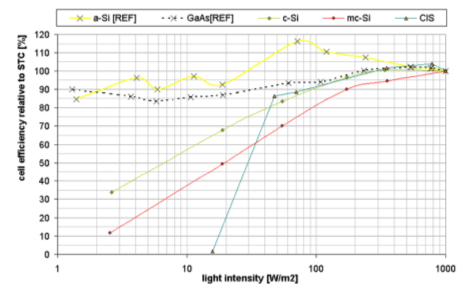
\includegraphics[scale=.5]{efficiency}
\caption{Efficienza di vari tipi di celle fotovoltaiche in funzione della luminosità incidente in \textit{Standard Test Condition}.}
\label{fig:efficiency}
\end{figure}

Infatti una cella fotovoltaica è schematizzata dal circuito equivalente in figura \ref{fig:equiv}. Pertanto una resistenza di shunt più alta, come nel caso del silicio amorfo, fa sì che una percentuale maggiore della fotocorrente generata (nello schema quella erogata dal generatore di corrente) passi nel circuito di carico e non rimanga nella fotocellula. Di fatti una delle caratteristiche per cui una cella fotovoltaica è considerata ideale è proprio a resistenza di shunt infinita.

\begin{figure}[htp]
\centering
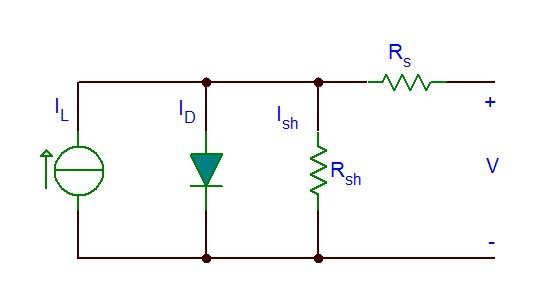
\includegraphics[scale=.5]{model}
\caption{Circuito equivalente di una cella fotovoltaica.}
\label{fig:equiv}
\end{figure}

Il modello si Shockley insieme alla conservazione della carica forniscono il seguente sistema di equazioni per la descrizione del circuito:

\begin{equation}
I_D = I_0 \, \Bigl(e^{\frac{q(V-IR_s)}{kT}}-1\Bigr)
\end{equation}

\begin{equation}
I = I_L - I_D - \frac{V-IR_s}{R_{sh}}
\end{equation}

\section{Misura della caratteristica I-V di una cella fotovoltaica}

Abbiamo simulato il circuito con TINA secondo lo schema in figura \ref{fig:simul}, ottenendo i grafici per le caratteristiche I-V e P-V al variare della resistena del potenziometro.

\begin{figure}[htp]
\centering
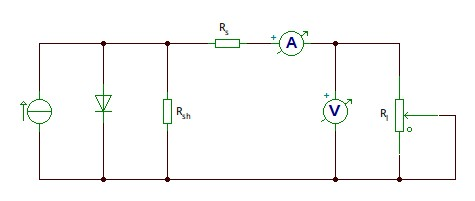
\includegraphics[scale=.4]{simul}
\caption{Circuito per la simulazione con TINA}
\label{fig:simul}
\end{figure}

In figura \ref{fig:ivchar} e \ref{fig:pvchar} sono riportati i grafici simulati, in cui si è posto $I_L = 10$ mA, $R_{sh}$ = 5 k$\Omega$, $R_s$ = 10 $\Omega$ e la resistenza è stata variata da 0 a 500 $\Omega$ (che corrisponde con il range di resistenze ottenibili con il potenziometro disponibile in laboratorio). Dalla caratteristica P-V si nota che per un certo valore della resistenza di carico si ha un massimo per la potenza erogata dalla cella. Tale resistenza la si ottiene dal rapporto $\frac{V}{I}$ alla corrispondente tensione.

\begin{figure}[htp]
\centering
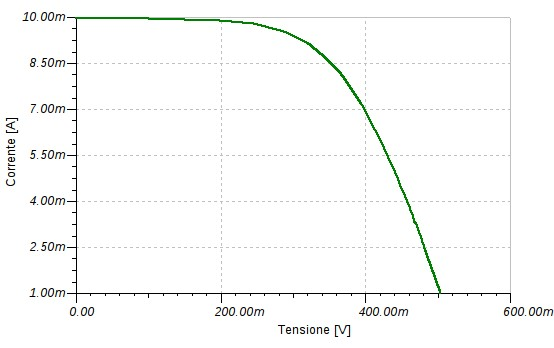
\includegraphics[scale=.4]{ivchar1}
\caption{Caratteristica I-V simulata della cella fotovoltaica}
\label{fig:ivchar}
\end{figure}

\begin{figure}[htp]
\centering
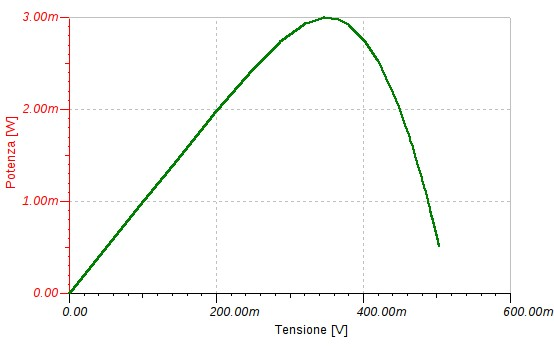
\includegraphics[scale=.4]{pvchar1}
\caption{Caratteristica P-V simulata della cella fotovoltaica}
\label{fig:pvchar}
\end{figure}

All'aumentare della resistenza di shunt i grafici precedenti non cambiano molto, dal momento che la cella fotovoltaica si avvicina al comportamento ideale, già ben approssimato con i valori precedenti. Riducend tale resistenza a 100 $\Omega$ i grafici cambiano significativamente, come si vede in figura \ref{fig:ivchar2} e \ref{fig:pvchar2}. Chiaramente la potenza massima trasferita diminuisce poichè una quantità maggiore di corrente scorre sul ramo di shunt. Aumentando $R_s$ si ottengono effetti analoghi, con una potenza massima lteriormente diminuita (meno di 1 mW) e la caratteristica I-V diventa completamente lineare.\\

\begin{figure}[htp]
\centering
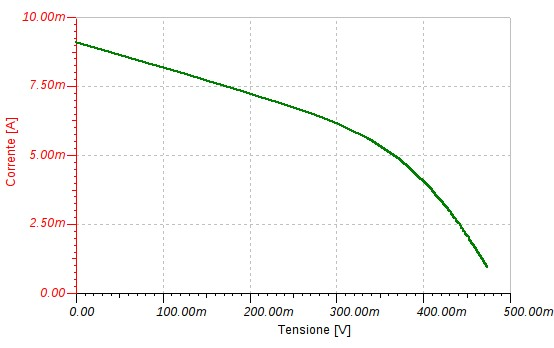
\includegraphics[scale=.4]{ivchar2}
\caption{aratteristica I-V simulata con $R_{sh}$ = 100 $\Omega$}
\label{fig:ivchar2}
\end{figure}

\begin{figure}[htp]
\centering
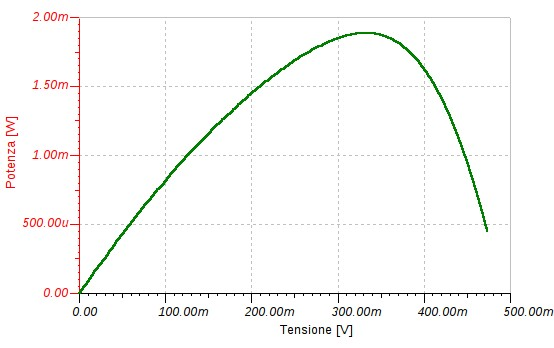
\includegraphics[scale=.4]{pvchar2}
\caption{Caratteristica P-V simulata con $R_{sh}$ = 100 $\Omega$}
\label{fig:pvchar2}
\end{figure}

Abbiamo realizzato infine sulla breadboard il circuito secondo lo schema in figura \ref{fig:mis}. Il potenziometro impiegato aveva come resistenza minima $R_{min} = 2.5(2) \Omega$ e come resistenza massima $R_{max}  = 502 \Omega \pm 0.8 \%$, abbiamo inoltre preso $R_1 = 2.5(1) \Omega$.\\

\begin{figure}[htp]
\centering
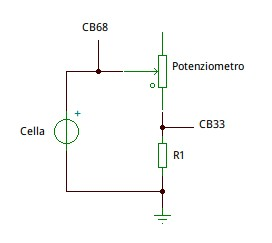
\includegraphics[scale=.6]{misura}
\caption{Schema del circuito realizzato sulla breadboard.}
\label{fig:mis}
\end{figure}

 Tramite il VI \texttt{Vin$\_$DC2ch} sono state acquisite le tensioni alla CB33 e CB68, la prima, nota $R_1$, fornisce la corrente che scorre nel circuito di carico, le seconda la tensione ai capi della cella. In tabella \ref{tab:cond} sono riportate le misure fatte con il VI in diverse condizioni.
 
\begin{table}
\centering
\caption{Valori di tensioni e correnti in varie condizioni.}
\label{tab:cond}
\begin{tabular}{|c|c|c|}
\hline 
Condizioni & Tensione (mV) & Corrente (mA) \\ 
\hline 
Luce lab & 88 & 0.205 \\ 
\hline 
Luce lab (res max) & 102 & 0.186 \\ 
\hline 
Luce lab (res min) & 2 & 0.540 \\ 
\hline 
Cella oscurata & 0 & 0.029 \\ 
\hline 
Led (res min) & 26 & 8.12 \\ 
\hline 
Led (res max) & 408 &  0.67\\ 
\hline 
Led (5 cm) & 287 & 0.488 \\ 
\hline 
Con flash (res min)& 32 & 9.81 \\ 
\hline 
\end{tabular} 
\end{table}

Come si vede da queste prime misure il comportamento della cella non contraddice l'andamento previsto, in particolare le misure fatte variando la resistenza del potenziometro.\\

Tramite il VI \texttt{Potenza$\_$celle} abbiamo tracciato la caratteristica I-V e P-V campionando le tensioni alle porte analogiche variando progressivamente la resistenza dell'amperometro. In figura \ref{fig:lab} sono mostrate le curve caratteristiche della cella alla luce ambientale. Come si vede  l'andamento ottenuto non coincide con quello in figura \ref{fig:ivchar}, ma è più lineare. A livello di simulazione con TINA si è verificato che nelle stesse condizioni, abbassando la corrente del generatore il grafico diventava sempre più lineare.

\begin{figure}[htp]
\centering
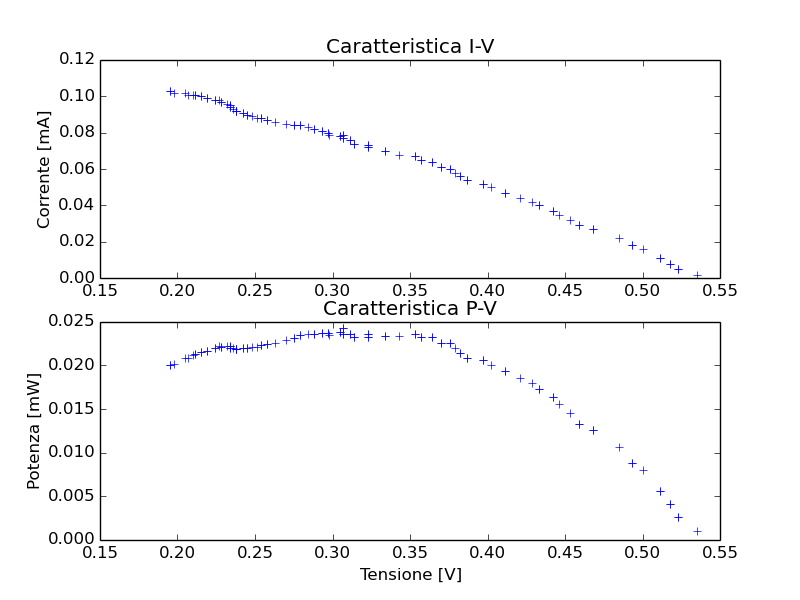
\includegraphics[scale=.45]{es4_luceamb}
\caption{Curve caratteristiche della cella alla luce del laboratorio.}
\label{fig:lab}
\end{figure}

Abbiamo fatto la stessa prova esponendo la cella alla luce di una lampada al led. Le curve ottenute si possono vedere in figura \ref{fig:led}. Questa volta il grafico è molto più simile a quello della prima simulazione, corrisponentemente alla maggiore fotocorrente generata.

\begin{figure}[htp]
\centering
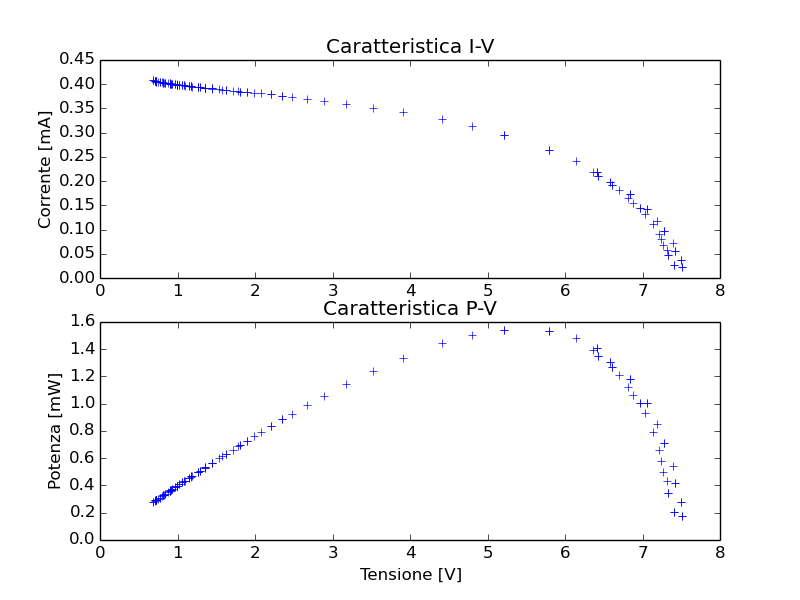
\includegraphics[scale=.45]{es4_luceled}
\caption{Curve caratteristiche della cella alla luce del laboratorio.}
\label{fig:led}
\end{figure}

Dai grafici è possibile ottenere una stima della resistenza di carico ottimale. Nel primo caso si ha che la potenza massima è erogata a V = 0.307(7) V, cui corrisponde una corrente di 0.075(3) mA, da cui la resistenza BOH
Nel secondo caso invece si ha V = 5.4(2) V e I = 0.28(1) mA, da cui R = BOH

%Lo, non tornano con quello che avevamo trovato, perché???????????????



\end{document}

